\PassOptionsToPackage{dvipsnames, table}{xcolor}
\documentclass[notitlepage, twocolumn, 12pt]{article}
\usepackage{mypackagesv2}
\usepackage{float}
\usepackage[tmargin=0.95in,bmargin=0.95in,lmargin=0.875in,rmargin=0.875in]{geometry}
\usepackage[dvipsnames]{xcolor}

\setlength{\belowcaptionskip}{-10pt}
\tolerance=1
\emergencystretch=\maxdimen
\hyphenpenalty=10000
\hbadness=10000

\title{Testing a Model to Predict the Motion of a Pendulum} 
\author{Pranav Upreti | PHY 180 Final Report}

\begin{document}
    \maketitle

    \section*{Introduction}
    A pendulum was constructed from household materials to test a damped harmonic oscillator model proposed by Brian Wilson \cite{Wilson}. Wilson's model was tested with four experiments in this lab. Part (i) tested Wilson's prediction of symmetry in the pendulum motion. To test this, the pendulum was released at different angles from the vertical and a period-angle graph was plotted was fit to $T_O(1+B\theta_0+C\theta_0^2$. The fit equation was (0.02 $\pm$ 0.04)$\theta^2$ - (0.003 $\pm$ 0.005)$\theta$ + 1.70 $\pm$ 0.03. The uncertainty on the coefficients of $\theta$ are greater than the coefficients themselves, so they are experimentally 0. This suggests the pendulum setup is symmetric because the release angle has negligible effects on period. 

    % TODO finish part 2,3,4. rename experiment parts to new naming. one column end. move some of discussion to uncertainty analysis

    Part (ii) used the same setup as part (i) to determine its $Q$ factor. The $Q$ factor is a constant which describes how quickly the pendulum's amplitude of oscillation decays (see background) and can be calculated two ways. First, by using the decay constant found by applying an exponential curve fit to an amplitude-time graph, and the relation $Q=\nicefrac{\pi\tau}{T}$, where $T$ is the period and $\tau$ is a decay constant found from the curve fit. It can also be counted by measuring the number of oscillations until the pendulum amplitude decays to $e^{-\pi}$ of its initial amplitude (see background) \cite{Wilson}. The pendulum's Q factor was measured to be 270 $\pm$ 20 from release angles between $1.40 \pm 0.01$ rad and $-1.40 \pm 0.01$ rad.
    
    Part (iii) used the same setup but varied the length of the pendulum string ($L$) and measured the pendulum's period ($T$). Wilson predicted that $T = 2 L^{0.5}$. The period-pendulum length data was fit to $T =kL^n$, where $k,n$ are constants and the best fit equation was found to be $T = (2.15 \pm 0.05)L^{0.44 \pm 0.06}$. The exponent on $L$ is consistent with Wilson's theory within the uncertainties, but the uncertainty on the coefficient of $L$ is not. 
    
    Part (iv) uses the data from part (iii) to plot $Q$ factor against pendulum length. It was fit against first and second order power series, exponential, and logarithmic functions.  Experimental results show the Q factor increased linearly with pendulum length by the equation $Q = (2.2 \pm 0.3)L + 80 \pm 10$. 
    
    The experimental results indicate that Wilson's model is most accurate for the range of angles tested. Quadratic damping forces like drag should be considered to improve this model. 

    \subsection*{Background}
    Pendulums and other oscillating systems decay in amplitude over time. Wilson suggests this is due to a damping force linearly proportional the velocity of the pendulum mass, call it $-b\diff{x}{t}$ where $b$ is a constant, $x$ is a particle's displacement from equilibrium, and $t$ is time \cite{OpenStax}. We use this to begin deriving Wilson's model:
    \begin{align*}
        m \diff[2]{x}{t} &= - b \diff{x}{t} - kx \\
        \intertext{where $b$ is some constant, and $k$ is the spring constant of the rope. Rearrange to obtain,}
        0 &= m \diff[2]{x}{t} + b \diff{x}{t} + kx   \\
    \intertext{this is a linear differential equation \cite{OpenStax} whose solution is} 
        x(t) &= A_0e^{\nicefrac{-bt}{2m}}\cos(\omega t + \phi)
    \end{align*} 
    Wilson's model is equivalent and predicts angle with time instead of position. As well, it introduces a constant $\nicefrac{1}{\tau} = \nicefrac{b}{2m}$ and uses $\omega = \nicefrac{2 \pi}{T}$ to get the equation:
    \begin{equation}\label{eq:1}
        \theta(t) = \theta_0 e^{-\nicefrac{t}{\tau}}\cos(\nicefrac{2\pi}{T} + \phi)
    \end{equation}
    The exponential decay in amplitude this model predicts is quantified by a constant called the $Q$ factor;  $Q \vcentcolon= \nicefrac{\pi \tau}{T}$. $Q$ can be calculated by finding $\tau$ from experimental data and substituting it into $Q = \nicefrac{\pi \tau}{T}$, or by measuring the number of oscillations until the amplitude of oscillation is $\theta_0e^{-\pi}$. Both methods were used to calculate $Q$. 
    
    \section*{Methodology} \label{method}

    A pendulum, shown in \cref{fig:setup}, was constructed to test for (i) symmetry in the pendulum setup, (ii) the $Q$ factor of the pendulum and (iii) a relationship between the length of the pendulum, the $Q$ factor, and the pendulum period.
    \begin{figure}[H]
        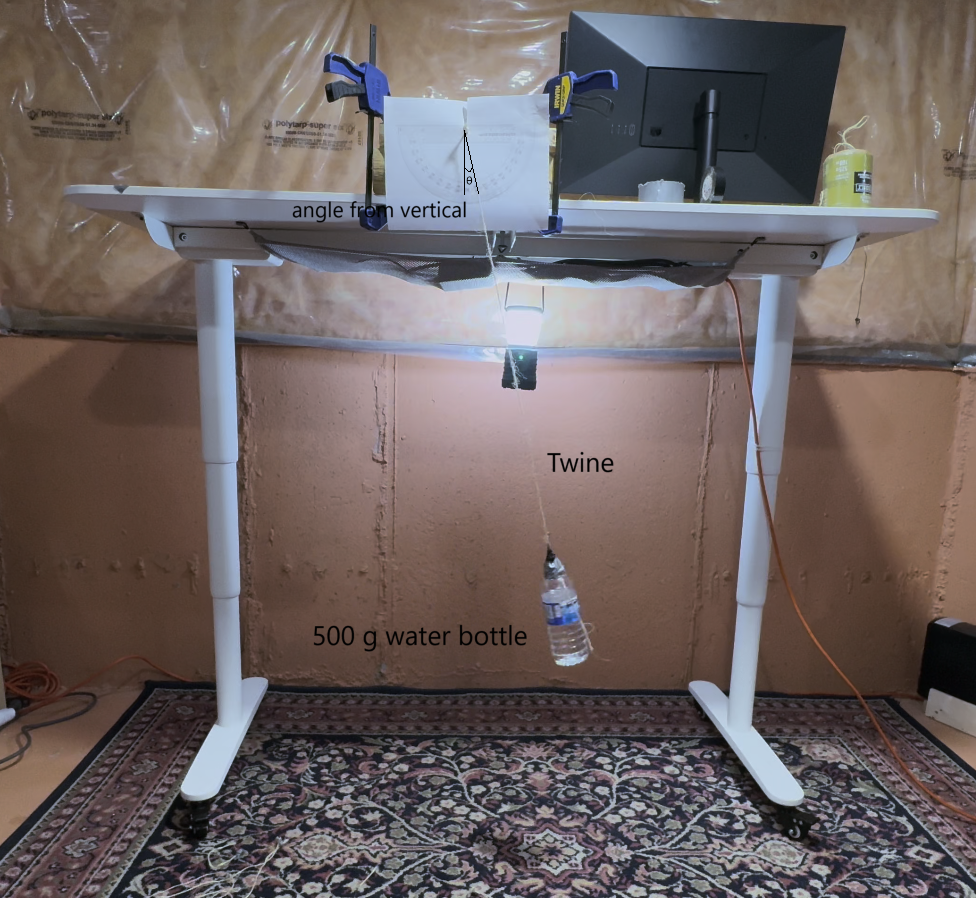
\includegraphics[width=\linewidth]{temp.png}
        \caption{The experimental setup}
        \label{fig:setup}
    \end{figure}
    For part (i), an 85.0 $\pm$ 0.5 cm jute twine string with mass $<$ 10.0 $\pm$ 0.1 g was tied from one end to a 500 mL plastic water bottle filled with water to a mass of 500.0 $\pm$ 0.1 g. The other end of the jute twine was tied to a nail 100.0 $\pm$ 0.5 cm above the ground. The jute twine was tied tightly so there was no visible slipping when the mass swung. To record the motion of the pendulum, a smartphone camera was positioned 120.0 $\pm$ 0.5 cm away from the pendulum setup. The camera recorded video at 30 FPS and its video was inputted into an application called \textit{Tracker} which automatically tracked the horizontal and vertical position of the pendulum with time. To calibrate the distance scale in the tracker application, a piece of 28.0 $\pm$ 0.5 cm paper was placed on the plane of the pendulum motion. The origin of the coordinate system was the center of the video frame. Black tape was placed on the water bottle to help the AutoTracker distinguish the water bottle from the light-coloured background. 
    Data from \textit{Tracker} was processed and graphed using a script provided by Wilson with some modifications (see Appendix).
    The mass was swung from 1.40 $\pm$ 0.01 rad to -1.40 $\pm$ 0.01 rad in increments of 0.35 $\pm$ 0.01 rad. The Tracker application plots a position-time graph, and the period was measured from this graph by taking the time it takes for 10 oscillations to complete and dividing by 10. This data is included in the Appendix and was processed to determine the relationship between release angle (part (i)). The same data was used to determine the Q factor of the pendulum (part (ii)).
    The experimental setup for part (iii) and (iv) is the same except the mass is swung from 0.52 $\pm$ 0.01 rad every trial, and the length of the string is varied from 20.0 $\pm$ 0.5 cm to 85.0 $\pm$ 0.5 cm. Additionally, a striped pattern of grey and black tape was added around the bottle to help AutoTracker identify a unique set of frames to track more accurately. All uncertainties in graphs were propagated by the code Wilson provided (see Appendix) 

    \section*{Part (i) Testing for Symmetry}
    Wilson's model suggests that the period of the pendulum is independent to the pendulum's release angle (Equation 1). The data is summarized in \cref{fig:symmetryTest}.

    \begin{figure}[H]
        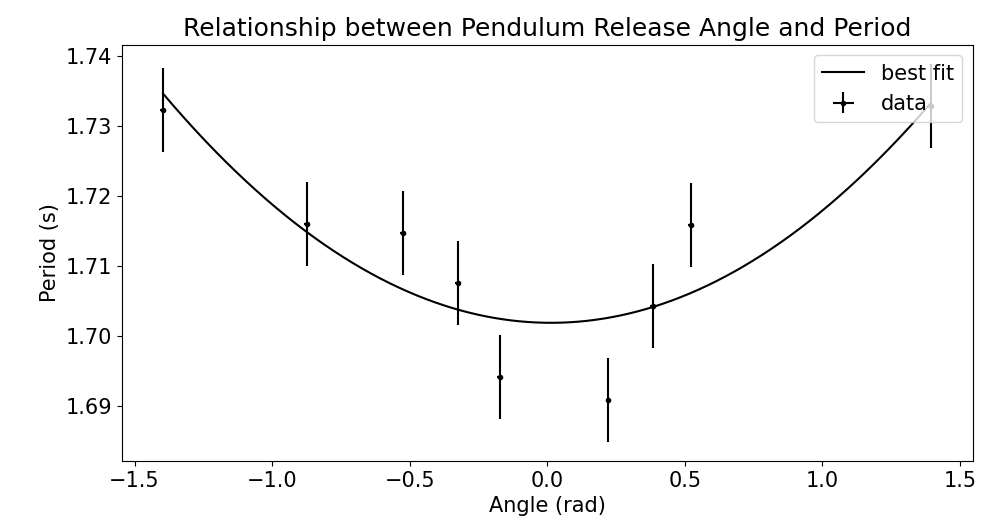
\includegraphics[width=\linewidth]{period_symmetry_revised.png}
        \caption{The period of the pendulum depend on the release angle from the vertical. The line of best fit as calculated by the provided Python code \cite{Wilson} was (0.02 $\pm$ 0.04)$\theta^2$ - (0.003 $\pm$ 0.005)$\theta$ + 1.70 $\pm$ 0.03. Horizontal error bars are not visible at this scale.}
        \label{fig:symmetryTest}
    \end{figure}

    % TODO: mention source of error and say as with... 
    \subsection*{Analysis and Uncertainties}
    \cref{fig:symmetryTest} suggests that the pendulum depends on the release angle from the vertical. Importantly, since the curve fit has a second order term, $-\theta$ and $\theta$ have the same period indicating that the setup is symmetrical. Note that for the first and second order terms, the uncertainty is greater than its value. We deduce that these values are experimentally zero, which suggests that the period of a pendulum is effectively constant. This deduction is valid for data range tested, which is important to consider because larger release angles make the pendulum mass swing faster, meaning quadratic drag forces may affect the period independence from release angle.

    Both type A and type B uncertainties were considered. For period measurements, the type A uncertainty was calculated as the standard deviation in period across 5 trials of one data point. The type B uncertainty is the length of a quarter frame (as taught in class), which equals $1/120 \rm{s} = 0.008 \rm{s}$. I multiplied this uncertainty by 8 ($0.008 \times 8 = 0.06$, or the length of two frames). This accounts for human error because I had difficulty pinpointing when the pendulum period endpoint. The Type A uncertainty in release angle was 0 since the pendulum mass was set to the same angle each trial. The type B uncertainty came from the protractor which measured in increments of $2^\circ$, which meant the uncertainty was $0.5^\circ = 0.009$ rad. 
    For both the period and angle measurements, the type B uncertainty was greater than the type A uncertainty, so that value was used. 

    The largest source of error comes from the pendulum moving in the axis into the page of \cref{fig:setup}. I tried minimizing this by constraining the pendulum motion with tape at the rotation point, but there was always some off-axis motion. The effect on experimental results cannot be easily quantified without knowing more initial conditions (i.e. angle of pendulum in the $\hat{z}$ direction). The practical way to minimize this error next time is to have the pendulum mass rotate about a hinge, which would constrain any off-axis motion.  
    \section*{Part (ii) Empirically determined Q factor}
    In part (i) we found that the release angle of the pendulum is approximately independent to its period. So, any part (i) trial can be used to calculate $Q$ and I chose an angle 0.34 $\pm$ 0.01 rad because it was easy set up.

    $Q$ is related to the exponential decay of amplitude with time so amplitudes of any position-time graph were plotted and an exponential best fit line was drawn (\cref{fig:amplitudeTgraph}). 

    \begin{figure}[H]
        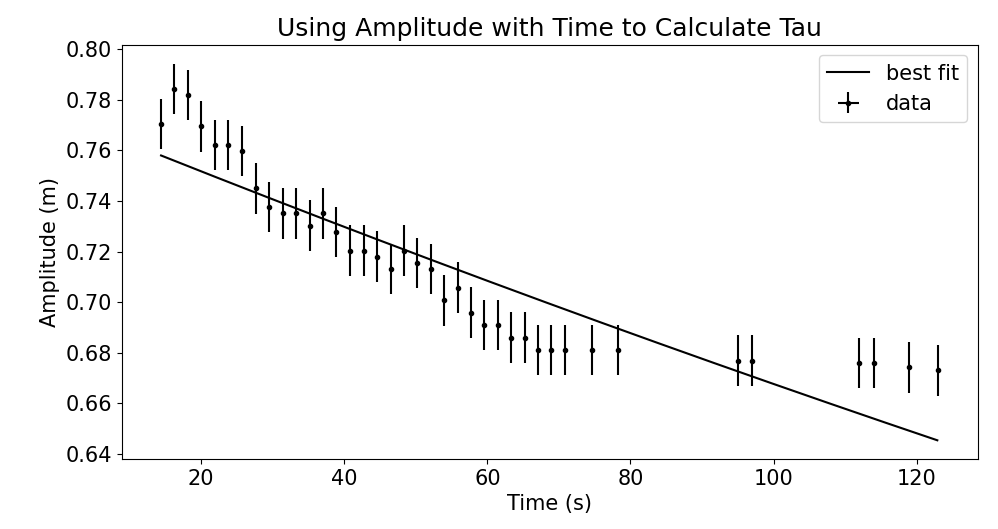
\includegraphics[width=\linewidth]{suspicious_tau_graph.png}
        \caption{Graph of amplitude (m) vs time (s) was fit to an exponential curve fit (it appears to be a straight line because of the scale). The best fit equation was (0.774 $\pm$ 0.004)$e^{-\nicefrac{t}{700 \pm 100}}$, which means $\tau$ = 700 $\pm$ 100 s.  Horizontal error bars come from the uncertainty in period ($\pm 0.03 s$) are too small to be seen. The vertical error bars were calculated as half the width of the bottle cap.}
        \label{fig:amplitudeTgraph}
    \end{figure}

    \subsection*{Uncertainties and Analysis}
    We used the experimental $\tau$ value to calculate the Q factor. Recall that $Q = \nicefrac{\tau \pi}{T} = \nicefrac{700\pi}{T} \pm (\nicefrac{100}{700})\times 100\% = 1300 \pm 200$. A Q factor of 270 $\pm$ 20 was also determined by counting the number of periods until the amplitude is $e^{-\pi}=4\%$ of its original amplitude. Since the Q factor is proportional to time, its percentage uncertainty matches the uncertainty in time.
    
    The two methods of calculating the Q factor give significantly different results, even while considering their uncertainties. I chose to use the counting method because the equation method assumes Wilson's theory is correct, but the counting method only assumes the pendulum motion is periodic. % unclear justification 

    For the uncertainties in amplitude of period, the type A uncertainty was the standard deviation across 5 trials, which was smaller than the type B uncertainty. It was calculated as half the width of the bottle cap = 24 mm / 2 = 12 mm $\approx$ 0.01 m. This uncertainty is reasonable since Tracker tracked pixels on the bottle cap, so it could be at most 12 mm away from the pendulum center. The uncertainty in period was calculated as the length of one frame, which is $0.03$ s; I scrubbed the video two frames at a time, so the period is likely off by at most one frame.

    The largest source of error comes the pendulum mass moving off-axis. This means some energy goes to wobbling the pendulum mass so the pendulum motion decays quicker in the plane we measured it from. This reduces the value of Q; the effect can be minimized as explained in Part (i). 

    Another source of error comes from my choice of target pixels used by AutoTracker. I used the top of the bottle cap to track pixels instead of the center mass, which Wilson's model is based off, because the water bottle cap tracked better (tracking from the center of mass skipped many frames). This likely has negligible effect on the experimental results because the period of the pendulum is the same for any point on the water bottle as long as it remains a rigid body, which it did.
    
    \section*{Part (iii) Relationship between Pendulum Length and Period}
    The pendulum mass was released from 0.52 $\pm$ 0.01 rad from the vertical at 5 different pendulum lengths and the data is summarized in \cref{fig:pendulumLengthVsPeriod}.
    \begin{figure}[H]
        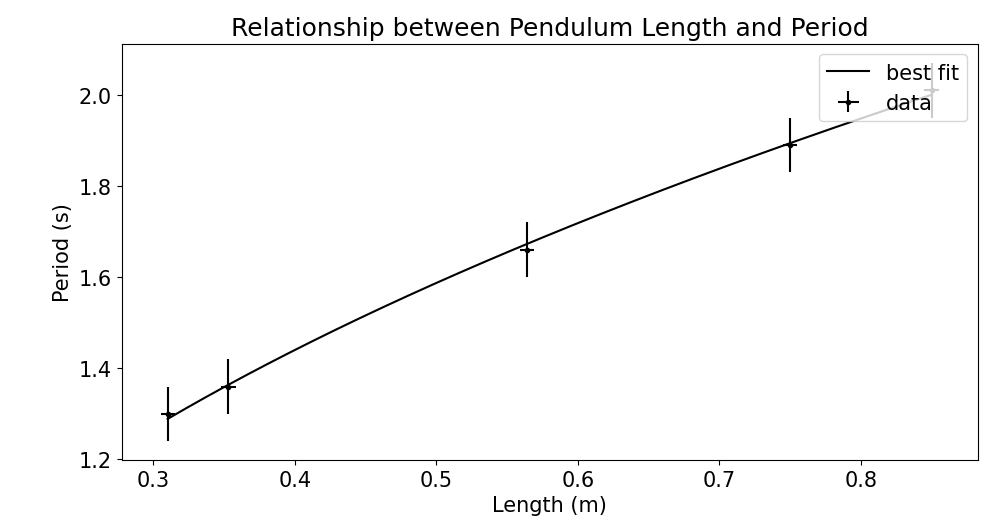
\includegraphics[width=\linewidth]{lengthvsperiodreal.png}
        \caption{Graph of period vs. pendulum length (m) with a power law fit shows $T = (2.15 \pm 0.05)L^{0.44 \pm 0.06}$. Horizontal error bars come from uncertainty in length which equals 0.005 m (half the smallest increment of the measuring tape used), and is too small to be seen. The vertical error bars are the uncertainty in period, 0.06 s. }
        \label{fig:pendulumLengthVsPeriod}
    \end{figure} 
    The same data was also plotted on a log-log scale:
    \begin{figure}[H]
        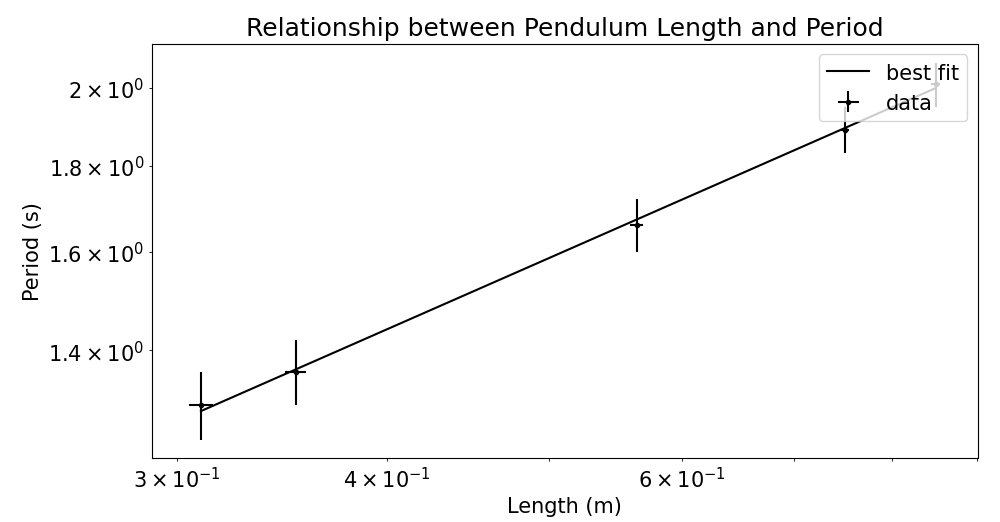
\includegraphics[width=\linewidth]{loglong-lengthvsperiodv2.png}
        \caption{Graph of period vs. pendulum length (m) on a log-log scale. The log-log graph has a y-int of $2.15 \pm 0.05$ and slope of $0.44 \pm 0.06$. Horizontal error bars are too small to be seen, and the vertical error bars is the uncertainty in period. }
        \label{fig:loglog-pendulumLengthVsPeriod}
    \end{figure} 

    Compared to exponential, linear, and quadratic fits, the power law fit passed through the most error bars so was the most suitable curve fit function.

    \subsection*{Uncertainties and Analysis}
    Wilson predicted the power law best fit function to be $T = kL^n = 2L^{0.5}$. Our power law curve fit is $T = (2.15 \pm 0.05)^{0.44\pm 0.06}$. This disagrees with Wilson's prediction that $k = 2$ but agrees with $n=0.5$ within the uncertainties.  This data suggests that either Wilson's model is wrong by factor (perhaps damping force is a calculable constant), or there is a systematic error not accounted by uncertainties caused by the pendulum setup. 

    Type A uncertainties were once again tiny compared to type B uncertainties, because of a small standard of deviation between the results of 5 trials. Type B uncertainties in period are calculated in the same manner described in part (ii). The type B uncertainty in length was half the smallest increment of the measuring tool (measuring tape) = $\nicefrac{1}{2}\times 1$ cm. I used half instead of a quarter we learned in class because my measuring tape was not perfectly in line with the pendulum setup because of the size of setup. This uncertainty can be reduced by accounting for parallax error.

    Additional sources of error come from off-axis wobble and AutoTracking not tracking the center of mass are prevalent as explained in Parts (i) and (ii). We can expect that the wobbling-off-axis error reduces the period of the pendulum since energy is lost to wobble, so the pendulum period is smaller. This suggests that the $2.15 \pm 0.05$ term is too low (the exponential term is likely not affected since the decay rate should remain similar; the error reduces the period of all data points.)

    \section*{Part (iv) Relationship between Pendulum Length and Q Factor}
    The data obtained in part (iii) was used to calculate $Q$ for pendulum length using the counting method. The counting method, described in part (ii) was used because it is more reasonable for the data used.  $Q$ factor was graphed against pendulum length and a linear, quadratic, and exponential fit were applied. The linear fit was the appropriate fit since it passed through the most error bars. 
    \begin{figure}[H]
        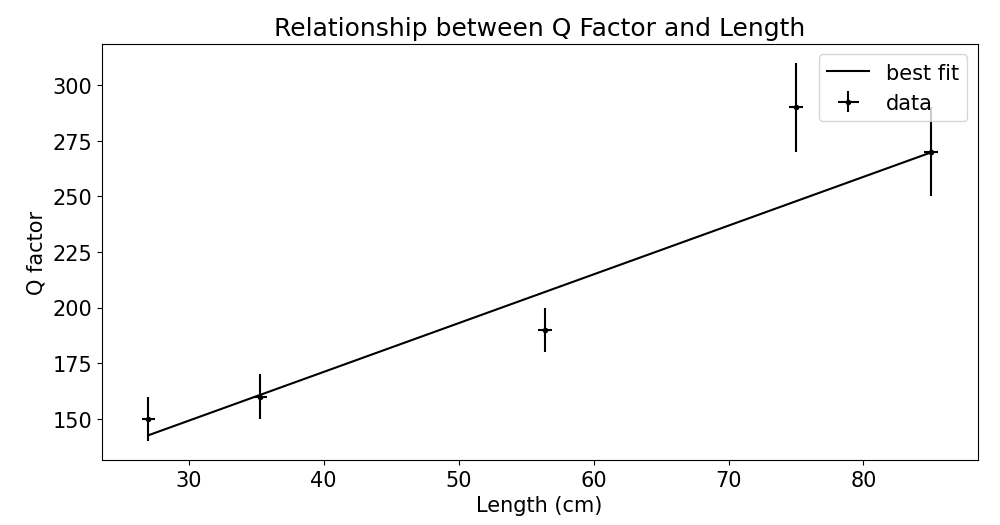
\includegraphics[width=\linewidth]{qfactorvslength.png}
        \caption{Graph of Q factor vs. pendulum length (cm) with a linear fit shows that the Q factor scales linearly with the length of the pendulum. Horizontal error bars is the uncertainty in length and the vertical error bars is the uncertainty in $Q$ factor. The best fit line is $Q = (2.2 \pm 0.3)L + 80 \pm 10$, where $L$ is the length of the pendulum.  }
        \label{fig:qfactorvslength}
    \end{figure} 

    \subsection*{Uncertainties and Analysis}
    The $Q$ factor increases with pendulum length by the relation $Q = (2.2 \pm 0.3)L + 80 \pm 10$. However, the point at  75.0 $\pm$ 0.5 cm does not follow the linearly increasing trend. This data point could be a measurement error, but that is unlikely since multiple trials were taken. We conclude a greater range of lengths needs to be measured to develop a conclusive relation between $Q$ factor and pendulum length.  

    The type A and type B uncertainties are the same for part (iii). Since $Q$ factor is proportional to time, the percentage uncertainties for time were used as percentage uncertainties of $Q$. Next time to reduce uncertainty, a higher frame rate camera could be used since it was noted in part (ii) that the uncertainty in time came from difficulty pinpointing the end of the period. A higher frame rate camera would make the motion smoother and easier to pinpoint. 

    Additional sources of errors are the same as Part (iii) since Part (iv) uses the same data.

    \section*{Conclusion}
    This experiment was split into four parts to test the validity of Wilson's model that predicts the behaviour of a pendulum. Data was obtained from a pendulum constructed from homemade materials. 
    
    In part (i) we found that the relationship between period and release angle was given by $T=$ (0.02 $\pm$ 0.04)$\theta^2$ - (0.003 $\pm$ 0.005)$\theta$ + 1.70 $\pm$ 0.03. The coefficients on $\theta$ are experimentally zero when considering the uncertainty which matches Wilson's prediction that period is independent of release angle the tested -1.40 $\pm$ 0.01 rad to 1.40 $\pm$ 0.01 rad. 
    In part (ii), we determined the $Q$ factor for our pendulum was $270 \pm 20$ by the counting method or $1300 \pm 200$ which assumes Wilson's model is correct. The counting method was deemed more accurate since it does not rely on the validity of Wilson's model. The large discrepancy suggests Wilson's model is inaccurate in predicting the decay of a pendulum.
    In part (iii), an experiment found the relation between period and pendulum length to be $T = (2.15 \pm 0.05)^{0.44\pm 0.06}$ which differs from Wilson's model.
    In part (iv), $Q$ factor was plotted against pendulum length to get $Q = (2.2 \pm 0.3)L + 80 \pm 10$ from the most suitable curve fit function. One $Q$ data point decreased with length instead of increasing which suggests a greater data range is needed to make a conclusion about the $Q$ factor-length trend.
    
    The data suggests Wilson's model is partially correct; a better model would account for quadratic damping forces to provide insight on the difference between the theoretical model and the experimental results.

    \onecolumn
    \begin{thebibliography}{}

    \bibitem{OpenStax}
    OpenStax. (n.d.). \textit{15.5 Damped Oscillations | University Physics Volume 1}. Retrieved from \url{https://courses.lumenlearning.com/suny-osuuniversityphysics/chapter/15-5-damped-oscillations/}

    \bibitem{Wilson}
    Wilson. (2022). \textit{PHY180 Lab Project (2024)}. Retrieved from \url{https://q.utoronto.ca/courses/363836/files/32826310?module_item_id=6082503}

    \end{thebibliography}

    \section*{Appendix}
    All data and code is stored \href{https://github.com/PRU1/PHY180-pendulum-project}{here}.

\end{document}